\documentclass[./\jobname.tex]{subfiles}
\begin{document}
\chapter {Experiment 0: Serial Memetic JADE}
\label{chap:experimet_0}

This chapter describes the results obtained by the most basic adaption of JADE for solving \gls{pde}s. The algorithm used here builds on the concepts described in \cite{chaquet_using_2019}. Aside from substituting some parameters, the only main difference is the usage of JADE instead of a \gls{cma_es}. 

\section{Hypotheses}
A memetic algorithm was first mentioned by \cite{moscato_evolution_2000}. In essence, it is a hybridisation of a population-based evolutionary algorithm and a deterministic direct or local search. The pseudocode \ref{algo: memeticJADE} below shows the implementation of such a memetic JADE. At first, JADE performs the global search and places its population around the optimum. Than the Downhill Simplex (\gls{ds}) exploits this area. The budget of \gls{nfe} is split into two parts: JADE takes nearly all \gls{nfe} and leaves $2\cdot dim$ \gls{nfe} for the \gls{ds}. The SciPy implementation of the \gls{ds} is used (\cite{scipy_scipyoptimizefmin_2020}).

\begin{algorithm}[h]
	\SetAlgoNoLine
	\DontPrintSemicolon
	\SetKwFunction{FmJADE}{memeticJADE}
	\SetKwProg{Fn}{Function}{:}{}
	\Fn{\FmJADE{$\mathbf{X}$, $funct$, $minErr$, $maxFE$}}{
		$dim$, $popsize$ $\gets size(\mathbf{X})$\;
		$p \gets 0.3$\;
		$c \gets 0.5$\;
		$pop$, $FE$, $F$, $CR$ $\gets JADE($$\mathbf{X}$, $p$, $c$, $funct$, $minErr$, $maxFE - 2 dim$ $)$\;
		$bestIndex = argmin(FE)$\;
		$bestSol = pop[bestIndex]$\;
		$pop$, $FE$ $ = downhill\text{ }simplex($$funct$, $bestSol$, $minErr$, $2 dim)$\;
		\Return $pop$, $FE$, $F$, $CR$
	}
	\unterschrift{Pseudocode of memetic JADE}{}{}
	\label{algo: memeticJADE}
\end{algorithm}

This experiment provides a first insight into the performance of the proposed algorithm. It tries to answer the question if JADE is a suitable surrogate algorithm for a \gls{cma_es}. Further, the memory usage and solving time is compared to the \gls{fem} results obtained in chapter \ref{chap:fem_baseline_results}. 

\section{Experiment Setup}
The standard parameters from table \ref{tab:ci_parameter} are taken. The memetic JADE is limited to either $10^4$ \gls{nfe} or $10^6$ \gls{nfe}. The experiment is done on two different machines. The first try with $10^4$ \gls{nfe} is run on the same machine ($\rightarrow$ machine 1) as the \gls{fem} experiment. This allows a fair memory and solving time comparison. This comparison can not be performed with the data obtained by using $10^6$ \gls{nfe} ($\rightarrow$ machine 2). Further, 5 \gls{gak} are used which results in a dimension of 20 parameters. Thus, the population consists of 40 individuals. 

To validate the results, a statistical significance test is performed. The test-function is based on the Wilcoxon test. The Wilcoxon test checks for significance at $\alpha = 0.05$. To decide if the results are better or worse, the mean and the median are compared. If both are smaller, the results are better. Contrary, if both are larger, the results are worse. If only one of the values is smaller, the results are undecided. The implementation is further explained in appendix \ref{chap:apendix_post_proc}. 

\section{Results}
\label{chap:experimet_0_results}
Table \ref{tab:results_literature_comparison} compares the obtained results with results from previous research papers. Therefore, the common testbed functions \gls{pde} 2 and \gls{pde} 3 are used. It is important to notice that the parameters used to obtain the results might not coincide. \cite{tsoulos_solving_2006} also use these two \gls{pde}s, but their paper did not provide any usable error metric. 
\begin{table}[H]
	\centering
	\noindent\adjustbox{max width=\linewidth}{
		\begin{tabular}{|c|c|c|c|}
			
			\hline
			\rowcolor[HTML]{\farbeTabA}
			
			Paper & Parameter & RMSE \gls{pde} 2 & RMSE \gls{pde} 3 \\ \hline
			\cite{chaquet_using_2019} & \multilinecell{4 kernel \\ max \gls{nfe}=$10^6$ \\ 50 replications } & $(1.75 \pm 1.14) 10^{-4}$ & $(1.09 \pm 0.846) 10^{-5}$  \\ \hline
			\cite{chaquet_solving_2012} & \multilinecell{10 harmonics \\ max \gls{nfe} = $G \cdot \lambda$ = $1.2 \cdot 10^6$ \\ 10 replications} & $(6.37 \pm 0.733) 10^{-3}$ & $(5.90 \pm 0.799)10^{-3}$ \\ \hline
			\cite{sobester_genetic_2008}& \multilinecell{50 max tree lenght \\ 12 generations \\ 20 replications} & $(6.9 \pm 8.3)10^{-4}$ & N/A \\ \hline
			\cite{panagant_solving_2014}& \multilinecell{unknowns: N/A \\ \gls{nfe}=$5\cdot 10^5$ \\ replications: N/A} & $7.256 10^{-4}$ & $9.489 10^{-6}$ \\ \hline
			serial memetic JADE & \multilinecell{5 kernel \\ max \gls{nfe} = $10^6$ \\ 20 replications} & $(2.9798 \pm 1.5541)10^{-2}$ & $(3.8225 \pm 1.9438)10^{-2}$ \\ \hline
			
		\end{tabular}
	}
	\unterschrift{This table compares the results obtained with the serial memetic JADE to the numerical results obtained by similar work in literature. The same metric must be used, thus the RMSE as defined in equation \eqref{eq:rmse_chaquet} is calculated.}{}{}
	\label{tab:results_literature_comparison}
\end{table}

The following table \ref{tab:serial_jade_compare_10^6_10^4} lists the smallest L2 norm reached after $10^4$ \gls{nfe} and $10^6$ \gls{nfe}, respectively. A standard Wilcoxon test, as described in the appendix \ref{chap:apendix_post_proc}, is performed. Remarkable is that the results on \gls{pde} 5 get significantly worse when more \gls{nfe} are used.  

\begin{table}[H]
	\centering
	\noindent\adjustbox{max width=\linewidth}{
		\begin{tabular}{|c|c|c|c|c|l|}
			
			\hline
			\rowcolor[HTML]{\farbeTabA}
			
			\gls{nfe} & \multicolumn{2}{|c|}{$10^4$} & \multicolumn{2}{|c|}{$10^6$} & \\ \hline
			stat & mean & median & mean & median & Wilcoxon Test \\ \hline \hline
			\gls{pde} 0A & 1.9415 $\pm$ 0.3321 & 1.8844 & 0.6596 $\pm$ 0.5510 & 0.9285 & sig. better \\ \hline
			\gls{pde} 0B & 0.7137 $\pm$ 0.1979 & 0.6354 & 0.2027 $\pm$ 0.1302 & 0.1516 & sig. better \\ \hline
			\gls{pde}  1 & 0.1874 $\pm$ 0.0408 & 0.1938 & 0.0149 $\pm$ 0.0049 & 0.0151 & sig. better \\ \hline
			\gls{pde}  2 & 0.0890 $\pm$ 0.0334 & 0.0760 & 0.0257 $\pm$ 0.0140 & 0.0224 & sig. better \\ \hline
			\gls{pde}  3 & 0.2409 $\pm$ 0.1051 & 0.2309 & 0.0328 $\pm$ 0.0169 & 0.0285 & sig. better \\ \hline
			\gls{pde}  4 & 0.1102 $\pm$ 0.0367 & 0.0985 & 0.0378 $\pm$ 0.0083 & 0.0352 & sig. better \\ \hline
			\gls{pde}  5 & 0.6645 $\pm$ 0.1930 & 0.6263 & 1.1968 $\pm$ 0.0286 & 1.2056 & sig. worse \\ \hline
			\gls{pde}  6 & 1.9660 $\pm$ 1.3845 & 1.6540 & 0.4135 $\pm$ 1.2133 & 0.0018 & sig. better \\ \hline
			\gls{pde}  7 & 0.0457 $\pm$ 0.0137 & 0.0452 & 0.0221 $\pm$ 0.0019 & 0.0223 & sig. better \\ \hline
			\gls{pde}  8 & 0.2186 $\pm$ 0.0045 & 0.2191 & 0.2170 $\pm$ 0.0019 & 0.2175 & unsig. better \\ \hline
			\gls{pde}  9 & 0.0525 $\pm$ 0.0147 & 0.0516 & 0.0451 $\pm$ 0.0119 & 0.0459 & unsig. better \\ \hline
			
		\end{tabular}
	}
	\unterschrift{L2 norm reached with serial JADE at $10^4$ \gls{nfe} and $10^6$ \gls{nfe}}{}{}
	\label{tab:serial_jade_compare_10^6_10^4}
\end{table}

The following two images \ref{fig:serial_jade_time_boxplot} and \ref{fig:serial_jade_memory_boxplot} show the time and memory usage for solving the testbed with $10^4$ \gls{nfe} in relation to the \gls{fem} solver. The images highlight the varying complexity of the testbed-\gls{pde}s and their corresponding fitness function. Although these results are not obtained for $10^6$ \gls{nfe}, they provide insight on how the solver scales with more \gls{nfe}. 

\begin{figure}[H]
	\centering
	\noindent\adjustbox{max width=0.66\linewidth}{
		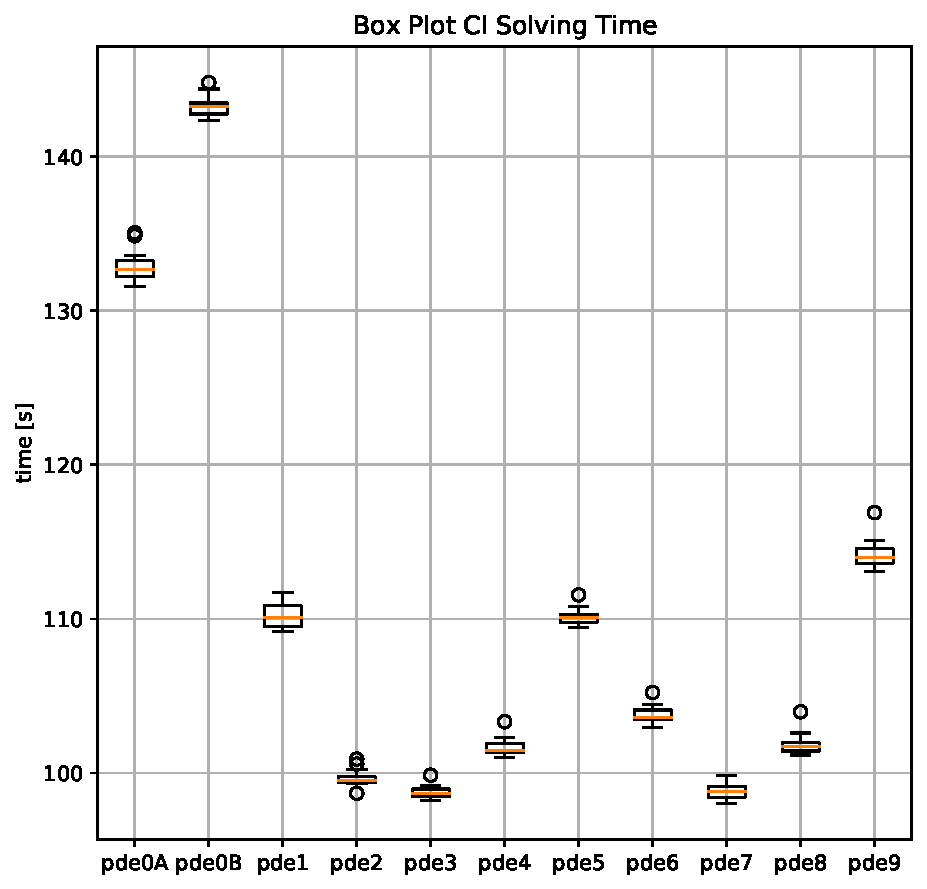
\includegraphics[width=\textwidth]{../../code/experiments/experiment_0/time_boxplot_ci_exp0.pdf}
	}
	\unterschrift{Relative solving time results of memetic JADE after $10^4$ \gls{nfe}.}{}{}
	\label{fig:serial_jade_time_boxplot}
\end{figure}


\begin{figure}[H]
	\centering
	\noindent\adjustbox{max width=0.66\linewidth}{
		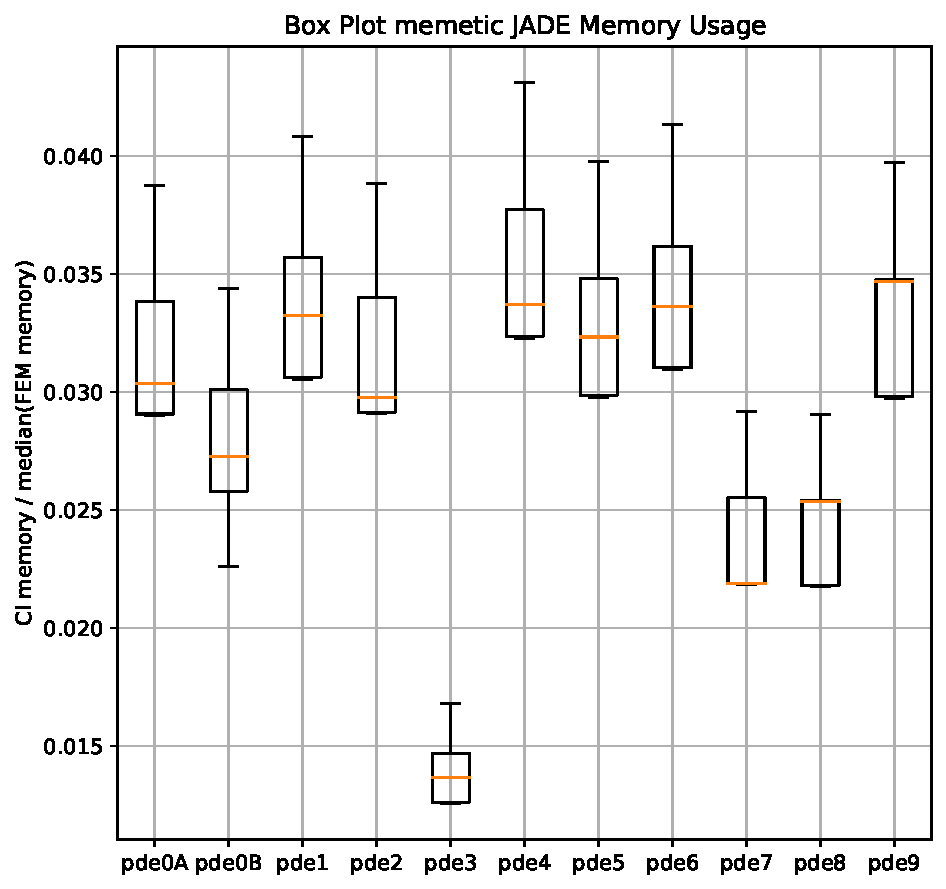
\includegraphics[width=\textwidth]{../../code/experiments/experiment_0/mem_boxplot_ci_exp0.pdf}
	}
	\unterschrift{Relative memory usage results of memetic JADE after $10^4$ \gls{nfe}.}{}{}
	\label{fig:serial_jade_memory_boxplot}
\end{figure}

\section{Discussion}

The results presented in chapter \ref{chap:experimet_0_results} above are discussed on the following pages. A comparison to the current literature is drawn. The solving time and memory consumption in relation to the \gls{fem} solver NGSolve is examined. Especially interesting are the results obtained on \gls{pde} 0A and \gls{pde} 5. 

\subsection{Comparison to Literature}

The \gls{rmse} reached on the \gls{pde} 2 and 3, are clearly not as good as the results obtained in previous papers, especially the results presented in \cite{chaquet_using_2019}. There might be a few reasons for that: 
\begin{itemize}
	\item As stated in the previous table \ref{tab:ci_parameter}, the penalty and weighting factor on the collocation points are different. These settings have been chosen on the basis of preliminary experiments, but there is no guarantee that the choice of these parameters is optimal. Setting these values is not a trivial task and must be tailored to the optimisation algorithm and the differential equation. 
	\item Since \gls{pde} 0A is defined as a combination of 5 \gls{gak}, at least so many kernels must be provided to the solver. This setup results in a greater search dimension, as compared in table \ref{tab:results_literature_comparison}. In general, more kernels result in a better solution, which is confirmed by experiments in \cite{chaquet_using_2019} and in chapter \ref{chap:pde 2 3 4 7}. 
	To reduce the computational effort per generation, and thus allow JADE to adapt the internal parameters for a longer period, the population size is set to $2 \cdot dim$. According to \cite{mallipeddi_empirical_2008}, the population size should not be lower than that. Again, choosing these parameters is not necessarily simple and the current setting could influence the convergence to the worse. 
	\item Compared to \cite{chaquet_using_2019}, the \gls{nfe}-budget for the local \gls{ds} search is smaller. Thus, the algorithm puts more emphasis on the exploration. However, due to the internal parameter-adaption JADE can perform both - exploration and exploitation. Preliminary experiments have shown that the direct search converges fast with very little progress after more than 100 \gls{nfe}.  
	\item JADE might simply be not as well suited for the problem as e.g. a \gls{cma_es}. 
\end{itemize}


%%%%%%%%%%%%%%%%%%%%%%%%%
%        time/mem       %
%%%%%%%%%%%%%%%%%%%%%%%%%

\subsection{Solving Time/Memory Usage}

The results from table \ref{tab:serial_jade_compare_10^6_10^4} show that the \gls{ci} solver can not nearly compete with the results obtained by the \gls{fem} solver from table \ref{tab:fem_sol_quality}. 
However, more interesting is the comparison of time and memory usage. 
In the current implementation, the population and the corresponding function values as well as the F and the CR history are recorded at every generation. Therefore, the memory usage scales linearly with the number of function evaluations used. This information is not necessary for the actual algorithm, but helpful for evaluating the results. In later implementations, this could be disregarded in order to even further reduce the memory consumption. Depending on the testbed \gls{pde}, only 1.5 to 4.0 percent of the memory used by the \gls{fem} solver is needed.

The \gls{ci} solver takes somewhere between 3 and 40 times as long as the \gls{fem} solver (figure \ref{fig:serial_jade_time_boxplot}) to perform $10^4$ \gls{nfe}. Since the solving time scales linearly, $10^6$ \gls{nfe} take about 10 times as long. More important, the \gls{ci} solver uses less memory on all problems (figure \ref{fig:serial_jade_memory_boxplot}). An interesting observation is the distribution of the solving time within the testbed. The more commands a fitness function needs, the longer is its solving time. However, this does not necessarily correspond with the quality of the solutions. For example, \gls{pde} 0B requires the longest absolute evaluation time ($29 \cdot 5 \text{ s} \approx 145\text{ s}$), compared to the other \gls{pde}s, it reaches a ``fairly'' good quality. 


%%%%%%%%%%%%%%%%%%%%%%%%%
%         PDE0A         %
%%%%%%%%%%%%%%%%%%%%%%%%%

\subsection{PDE 0A}
\label{chap: experiment_0_pde_0A}

The purpose of this \gls{pde} is to show that the solver would converge globally towards the analytical solution, if it can be represented by a finite number of kernels. However, his can not be confirmed with the current implementation. While more function evaluation do tend to generate better results (as confirmed by the Wilcoxon test in table \ref{tab:serial_jade_compare_10^6_10^4}), it is common for the \gls{ci} solver to result in different functions. A typical phenomenon is that the obtained approximation has some of its Gauss ``bumps'' outside of the domain $\Omega$. The comparison of two solutions with $10^4$ \gls{nfe} and $10^6$ \gls{nfe} in figure \ref{fig:serial_jade_pde0a_sol_comparison} shows this behaviour. Since the results improve from $10^4$ to $10^6$, it is possible that the results from $10^6$ \gls{nfe} can be refined with an even larger \gls{nfe} budget. However, this is not tested due to the already extensive computational effort. 

\begin{figure}[H]
	\centering
	\begin{subfigure}[b]{0.45\linewidth}
		\centering
		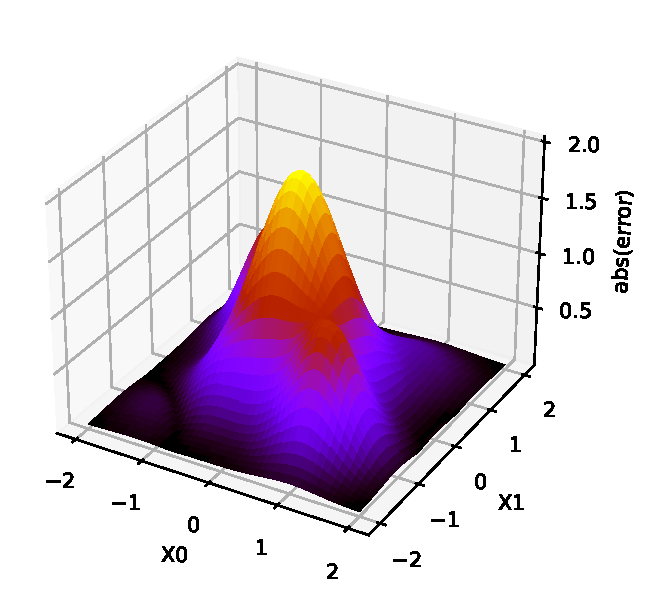
\includegraphics[width=1\textwidth]{../../code/experiments/experiment_0/pde0a_missing_bump_sol_10_4.pdf}
		\caption{\gls{pde} 0A error; $10^4$ \gls{nfe}: \\ L2 norm: 2.5075 \\ FE value: 4.4129 \\ RMSE: 0.5699}
		\label{fig:pde0a_sol_10_4}
	\end{subfigure}% 
	%
	\begin{subfigure}[b]{0.45\linewidth}
		\centering
		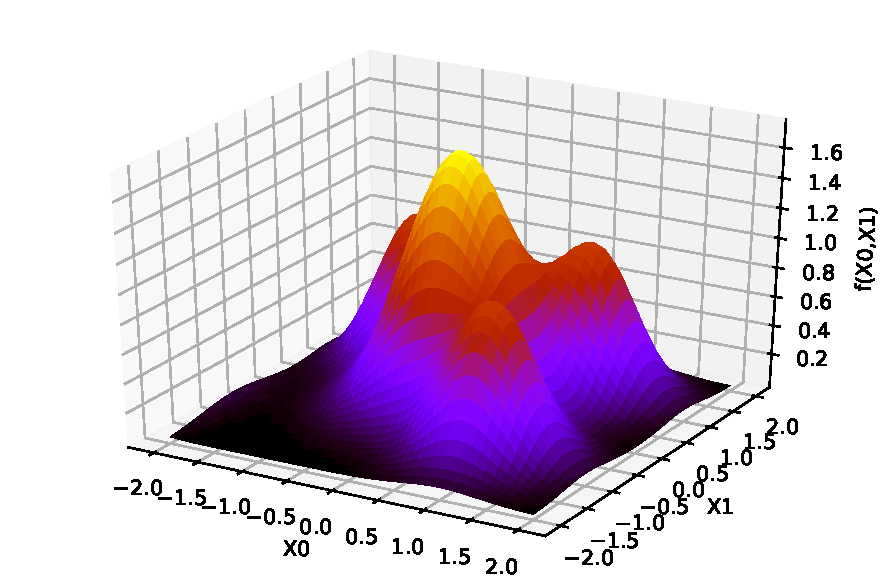
\includegraphics[width=1\textwidth]{../../code/experiments/experiment_0/pde0a_missing_bump_sol_10_6.pdf}
		\caption{\gls{pde} 0A error; $10^6$ \gls{nfe}: \\ L2 norm: 0.9281 \\ FE value: 1.3762 \\ RMSE: 0.2111}
		\label{fig:pde0a_sol_10_6}
	\end{subfigure}%
	\unterschrift{Comparison of two typical \gls{pde} 0A solutions. }{}{}%
	\label{fig:serial_jade_pde0a_sol_comparison}
\end{figure}


\subsection{PDE 5}
\label{chap:ex0_pde5}
%%%%%%%%%%%%%%%%%%%%%%%%%
%         PDE5          %
%%%%%%%%%%%%%%%%%%%%%%%%%
A fascinating property of \gls{pde} 5 is observed: more function evaluation (from $10^4$ to $10^6$) result in a significantly worse solution quality. This is confirmed by a Wilcoxon test, as seen in table \ref{tab:serial_jade_compare_10^6_10^4}. 
This property can even be concluded from a visual perspective. A comparison of the best solution after $10^4$ \gls{nfe} and the best solution after $10^6$ \gls{nfe} is shown in figure \ref{fig:serial_jade_pde5_sol_comparison}. The solution after $10^4$ \gls{nfe} describes the global structure more accurately. It seems that the correct description of the boundary points gets lost with more \gls{nfe}.

\begin{figure}[H]
	\centering
	\begin{subfigure}[b]{0.3333\linewidth}
		\centering
		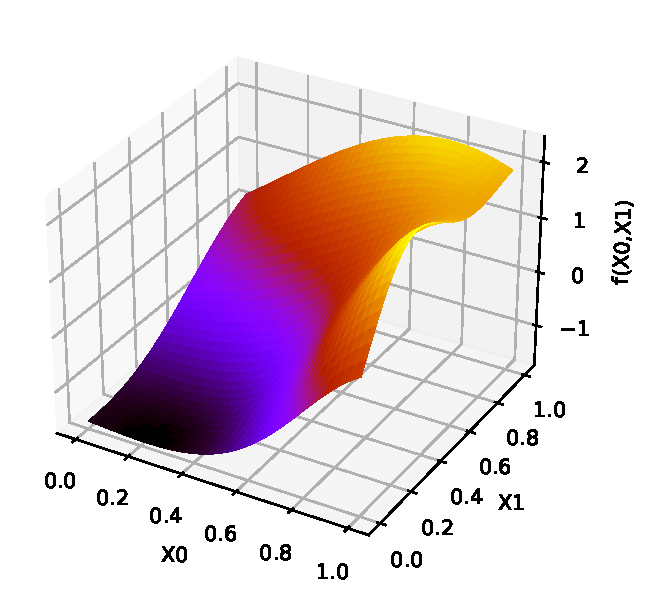
\includegraphics[width=1\textwidth]{../../code/experiments/experiment_0/pde5_best_sol_10_4.pdf}
		\caption{best solution $10^4$ \gls{nfe} \\ L2 norm: 0.4283 \\ FE value: 2980.96}
		\label{fig:pde5_sol_10_4}
	\end{subfigure}% 
	%
	\begin{subfigure}[b]{0.3333\linewidth}
		\centering
		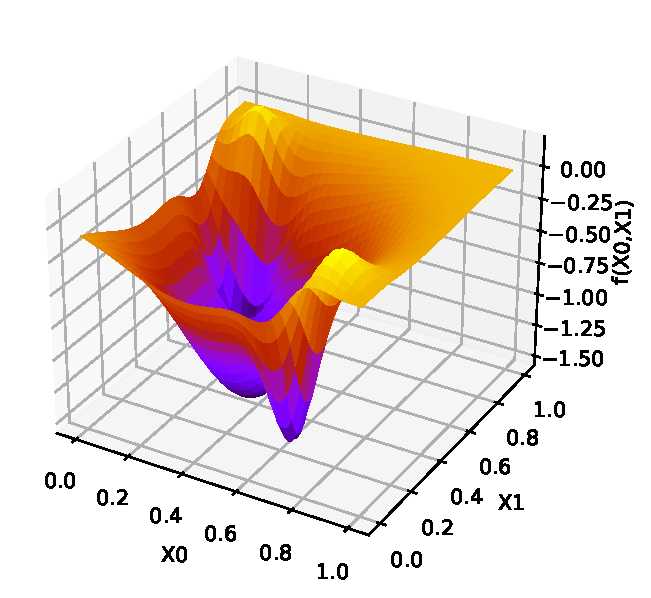
\includegraphics[width=1\textwidth]{../../code/experiments/experiment_0/pde5_best_sol_10_6.pdf}
		\caption{best solution $10^6$ \gls{nfe} \\ L2 norm: 1.1095 \\ FE value: 1007.44}
		\label{fig:pde5_sol_10_6}
	\end{subfigure}%
	%
	\begin{subfigure}[b]{0.3333\linewidth}
		\centering
		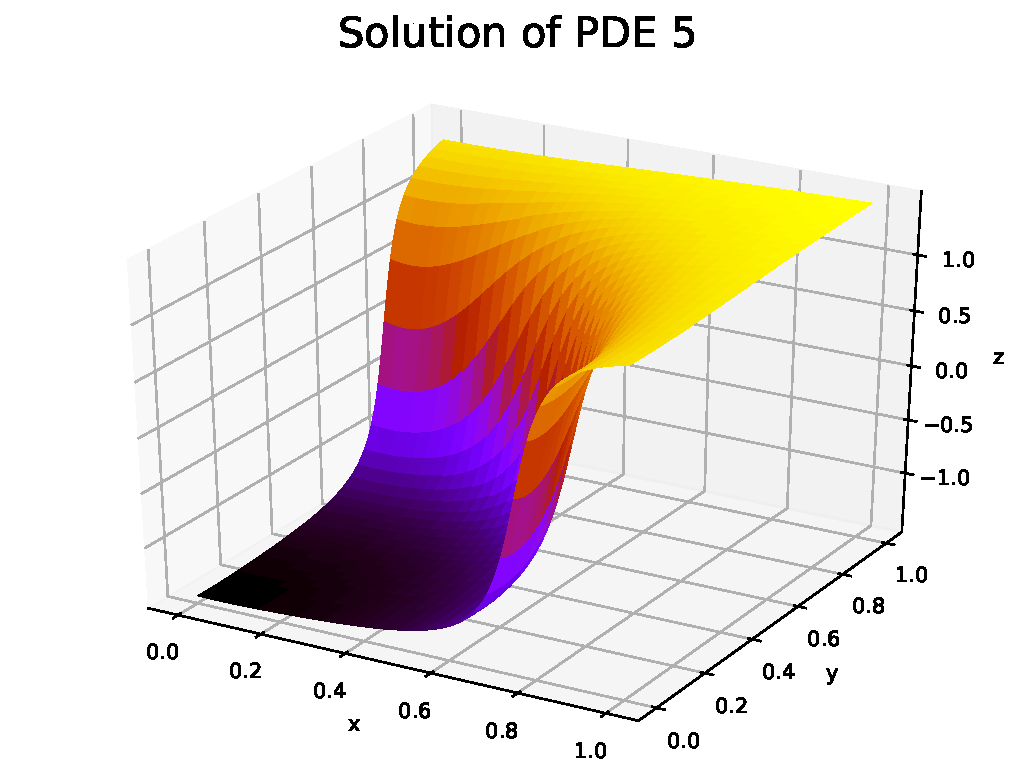
\includegraphics[width=1\textwidth]{../../code/testbed/pde5/sol_pde_5.pdf}
		\caption{analytical solution \\to testbed \\ \gls{pde} 5.}
		\label{fig:pde5_analytical_solution}
	\end{subfigure}%
	\unterschrift{Comparison of best solution after $10^4$ and $10^6$ \gls{nfe}.}{}{}%
	\label{fig:serial_jade_pde5_sol_comparison}
\end{figure}

The distributions of the achieved fitness value after $10^4$ and $10^6$ \gls{nfe} is shown in figure \ref{fig:pde5_fitness_histogram}. They are clearly separated with distinct mean and median. As expected, both the mean and the median after $10^6$ \gls{nfe} are significantly smaller than these values after $10^4$ \gls{nfe}. The corresponding L2 norm distributions are plotted in figure \ref{fig:pde5_norm_histogram}. As described by the Wilcoxon test, the results are inverted. The mean and the median of the L2 norm after $10^4$ \gls{nfe} are smaller than the ones after $10^6$ \gls{nfe}.

\begin{figure}[H]
	\centering
	\begin{subfigure}[b]{0.5\linewidth}
		\centering
		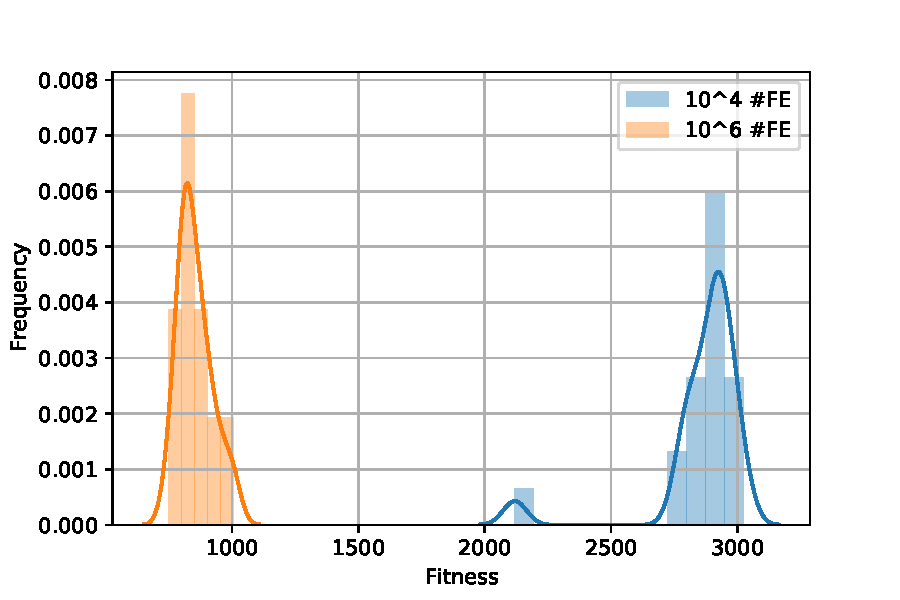
\includegraphics[width=1\textwidth]{../../code/experiments/experiment_0/pde5_fit_histogram.pdf}
		\caption{Histogram of the fitness value reached on \gls{pde} 5.}
		\label{fig:pde5_fitness_histogram}
	\end{subfigure}%
	%
	\begin{subfigure}[b]{0.5\linewidth}
		\centering
		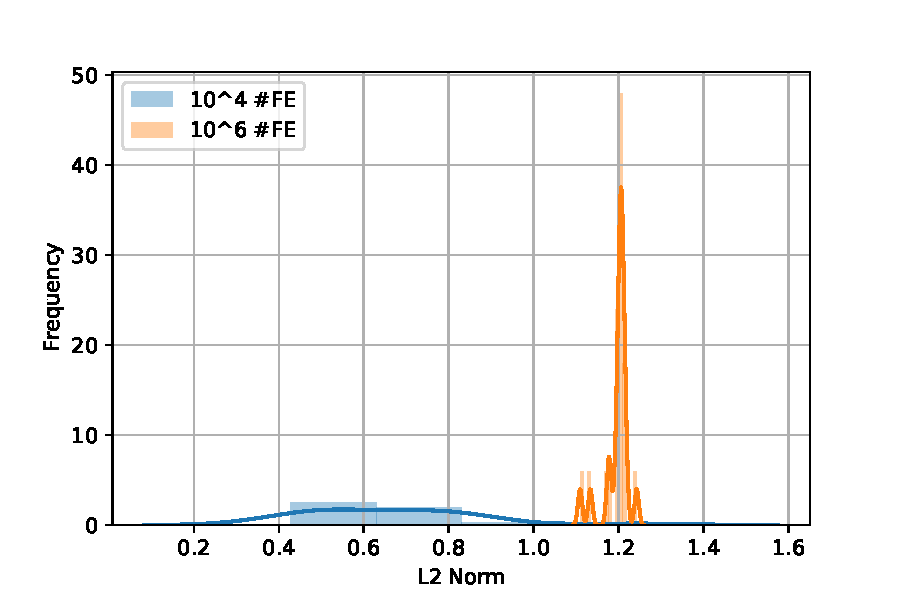
\includegraphics[width=1\textwidth]{../../code/experiments/experiment_0/pde5_norm_histogram.pdf}
		\caption{Histogram of the L2 norm reached on \gls{pde} 5.}
		\label{fig:pde5_norm_histogram}
	\end{subfigure}% 
	\unterschrift{Histograms of the fitness and the L2 norm reached with $10^4$ \gls{nfe} and $10^6$ \gls{nfe} on \gls{pde} 5.}{}{}%
	\label{fig:pde5_histograms}
\end{figure}

This phenomenon can be explained by the structural difference between the fitness function and the L2 norm. The fitness of a candidate solution can only decrease or stay the same, due to the greedy selection used in JADE (line 15 in the pseudocode \ref{algo: jade}). The monotonically decreasing fitness value at every generation of an exemplary individual within the population is plotted in figure \ref{fig:ex0_pde5_gak_fit_vs_l2}. Because the L2 norm is not the property that gets optimised, the quality of an individual at every generation is not necessarily monotonically decreasing. The corresponding L2 norm of the same individual is plotted alongside its fitness in figure \ref{fig:ex0_pde5_gak_fit_vs_l2}. 

\begin{figure}[H]
	\centering
	\noindent\adjustbox{max width=0.7\linewidth}{
		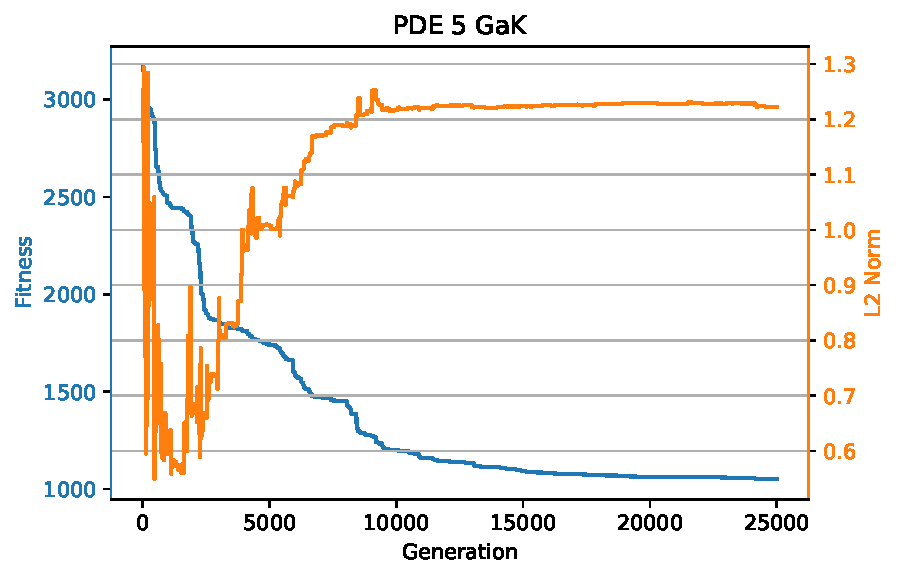
\includegraphics[width=\textwidth]{../../code/experiments/misc/pde5_gak_fit_l2_history.pdf}
	}
	\unterschrift{Fitness value and L2 Norm of one individual at every generation on \mbox{\gls{pde} 5.}}{}{}
	\label{fig:ex0_pde5_gak_fit_vs_l2}
\end{figure}

This indicates that the current fitness function does not fully describe the optimisation problem. Some possible solutions to this problem could be:
\begin{itemize}
	\item An adaptive number of kernels reduces the dimensionality of the problem and only increases the kernel number if necessary. 
	\item A different kernel type that better resembles the structure of the solution could be used. 
	\item A denser grid of collocation points alters the fitness function. This introduces more points that might sit at more interesting positions within the domain. However, this also increases the computational effort to evaluate the fitness function. Alternatively, a scheme that adapts the collocation points during the optimisation process could balance out the computational effort and interesting probing locations.
\end{itemize}

An adaptive kernel scheme is proposed in chapter \ref{chap:experimet_2}. The \gls{gsk} kernel type is examined in chapter \ref{chap:experimet_3}.

\end{document}